\documentclass{article}
\usepackage{amsmath}
\usepackage{amsthm}
\usepackage{amsfonts}
\usepackage{mathtools}
\title{MATH 618: Homework 3}
\author{Fernando}
\date{October 17, 2023}
\begin{document}
\maketitle
\section{Problem 1}
Let $T_nf\coloneqq\delta_{\frac{1}{n}}\cdot f$ where $\delta_{a}(x)=\begin{cases}
1 &\text{ if } x=a\\
0 &\text{ otherwise}
\end{cases}$, in other words:
\[ (T_nf)(x)=\begin{cases}
f(\frac{1}{n}) &\text{ if } x=\frac{1}{n}\\
0 &\text{ otherwise}
\end{cases}.
\]
$T_n$ is clearly linear because we are dealing with pointwise multiplication:
\[
T_n(cf+g)=\delta_{\frac{1}{n}}\cdot(cf+g)=c\delta_{\frac{1}{n}}\cdot
f+\delta_{\frac{1}{n}}\cdot g=cT_nf+T_ng
\]
Also it is easy to see that:
\begin{align*}
||T_n||_{\mathcal{A}}=\sup_{||f||_{L_\infty}=1}||T_nf||_{L_\infty}
&=\sup_{||f||_{L_\infty}=1} \left\{\sup_{x\in[0,1]}|T_nf|\right\}\\
&=\sup_{||f||_{L_\infty}=1} \left\{\left|f\left(\frac{1}{n}\right)\right|\right\}\\
&= 1
\end{align*}
So in effect $\{T_n\}\subset D$.
Now to prove that $\{T_n\}$ doesn't have any convergent subsequence we observe
that:
\begin{align*}
||T_n-T_m||_{\mathcal{A}}
&=\sup_{||f||_{L_\infty}=1}||T_nf-T_mf||_{L_\infty}\\
&\geq||T_ng-T_mg||_{L_\infty}\text{ (where $g\equiv 1$)}\\
&=\left|\left|\delta_{\frac{1}{n}}-\delta_{\frac{1}{m}}\right|\right|_{L_\infty}\\
&=\sup_{x\in[0,1]}\left|\delta_{\frac{1}{n}}-\delta_{\frac{1}{m}}\right|\\
&\geq \left|\delta_{\frac{1}{n}}(1/n)-\delta_{\frac{1}{m}}({1/n})\right|\\
&=|1-0|=1.
\end{align*}
Since this is for all $m,n$ we conclude that there cannot be any convergent
subsequence.
\section{Problem 2}
\subsection{Part a}
\textbf{Lema 1:} $\int_0^1 |\sin^{(k)}(n\pi x)|^2=cn^{2k}$, for
some constant c.

\textbf{Proof:} We proceed by induction over $k$ (technically strong
induction).

For $k=0$ we have:
$\int_0^1 |\sin^{(0)}(n\pi x)|^2=\frac{1}{2}n^{2\cdot 0}$.

Now for $k+1$ we have
\begin{align*}
\int_0^1 |\sin^{(k+1)}(n\pi x)|^2
&= \int_0^1 |n\pi\cos^{(k)}(n\pi x)|^2\\
&= \int_0^1 |n^2\pi^2\sin^{(k-1)}(n\pi x)|^2\\
&= n^4\pi^4\int_0^1 |\sin^{(k-1)}(n\pi x)|^2\\
&= n^4\pi^4cn^{2(k-1)} \quad \text{(by Induction Hypothesis)}\\
&= cn^{2(k+1)}.
\end{align*}
Which concludes the proof of lema 1.
Now we remember the fact that $H^k$ is a Hilbert space with the inner product
\[
	\langle u,v\rangle_{H^k} = \int uv + \int u'v' + \cdots + \int u^{(k)}v^{(k)}
\]
Then if we write $u\in L^2$ as $u=\sum a_n\sin(n\pi x)$ we get that
\begin{align}
	\langle u,u\rangle_{H^k} &= \Big\langle \sum a_n\sin(n\pi x), \sum a_n\sin(n\pi x) \Big\rangle_{H^k}\nonumber\\
	\langle u,u\rangle_{H^k} &= \sum_{n,m}\langle a_n\sin(n\pi x),
	a_m\sin(m\pi x) \rangle_{H^k}\nonumber\\
	\langle u,u\rangle_{H^k} &= \sum\langle a_n\sin(n\pi x), a_n\sin(n\pi x) \rangle_{H^k}\nonumber\\
	\langle u,u\rangle_{H^k} &= \sum ||a_n\sin(n\pi x)||^2_{H^k}\nonumber\\
	\langle u,u\rangle_{H^k} &= \sum a_n^2||\sin(n\pi x)||^2_{H^k}\label{convergence}.
\end{align}
In other words, if we want $u\in H^k$ we need its Fourier coefficients (namely
$a_n$) to converge to 0 fast enough to make (\ref{convergence}) convergent.
Using the lema we see that $||\sin(n \pi x)||^2_{H^k}$ has the form
\[
	\sum_{i=0}^k c_in^{2i}.
\]
Putting this together we conclude the Following:

\textbf{Conclusion:} Let $a_n$ be the Fourier coefficients of $u$, then $u\in
H^k$ if and only if the series:
\[
	\sum n^{2k}a_n^2
\]
is convergent.
\subsection{Part b}

\begin{figure}[ht]
\caption{Plot of $u_0$}
\centering
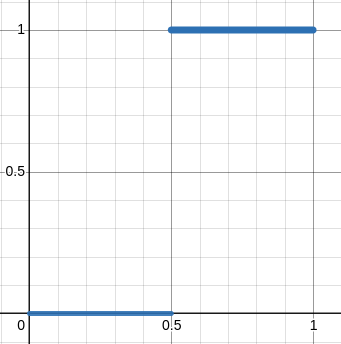
\includegraphics[width=0.5\textwidth]{u_0.png}
\end{figure}
\begin{figure}[ht]
\caption{Plot of $u_1$}
\centering
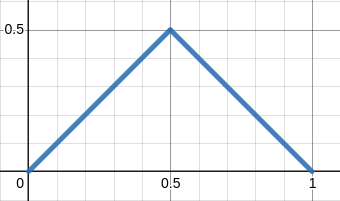
\includegraphics[width=0.5\textwidth]{u_1.png}
\end{figure}
\begin{figure}[ht]
\caption{Plot of $u_2$}
\centering
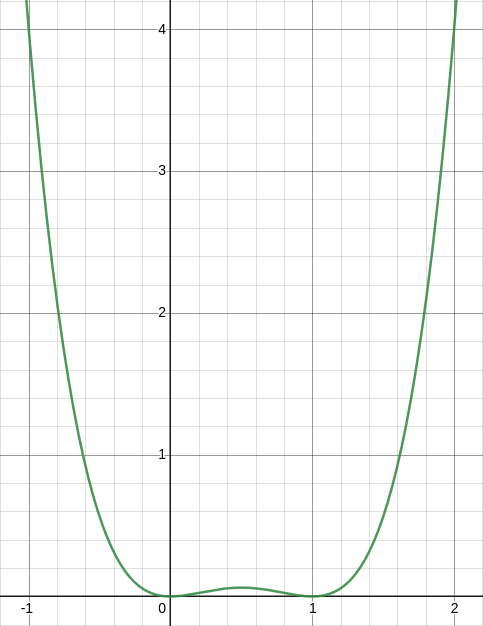
\includegraphics[width=0.4\textwidth]{u_2.png}
\end{figure}
\begin{figure}[ht]
\caption{Plot of $u_\infty$}
\centering
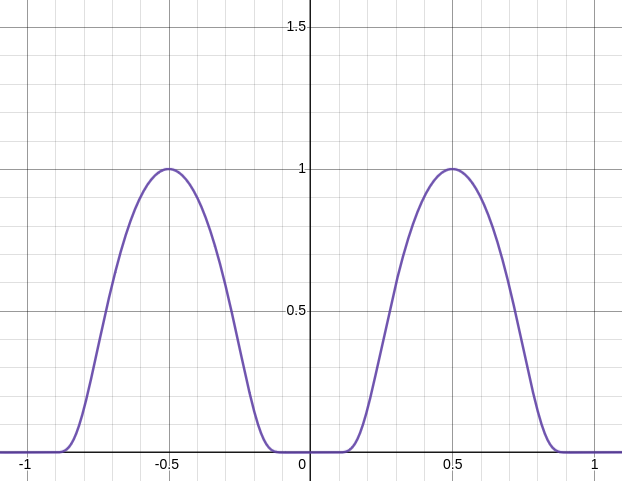
\includegraphics[width=0.5\textwidth]{u_inf.png}
\end{figure}
\newpage
\subsection{Part c}
Computing Fourier coefficients.
\subsection{$u_0$}
\begin{align*}
	a_n&=2\int_0^1 u_0(x)\sin(n\pi x)\\
	  &=2\int_{0.5}^1\sin(n\pi x)\\
	  &= -2\frac{\cos(n\pi x)}{n\pi}\Big|_{0.5}^1\\
	  &= \frac{2}{n\pi}\left(\cos\left(\frac{n\pi}{2}\right)-\cos(n\pi)\right)
\end{align*}
\subsection{$u_1$}
For this one if we try to compute the integral we get a messy thing so it is
better to exploit the symmetry of the functions around $\frac{1}{2}$.

We start by observing that for $n$ even we have
\[
\sin\left(n\pi \left(\frac{1}{2}-x\right)\right)=-\sin\left(n\pi \left(\frac{1}{2}+x\right)\right)
\]
i.e. $\sin$ is odd with respect to the
$x=\frac{1}{2}$ and also notice that $u_1$ is even with respect to
$x=\frac{1}{2}$, so for $n$ even
\[
a_n=2\int_0^1 u_1(x)\sin(n\pi x)=0.
\]
Now for $n$ odd we can show in the same way that $\sin(n\pi x)$ is even with
respect to $x=\frac{1}{2}$, then
\begin{align*}
	a_n&=2\int_0^1 u_1(x)\sin(n\pi x)\\
	  &=4\int_0^{0.5}x\sin(n\pi x)\\
	  &=4\left(\frac{\sin(n\pi x)-n\pi x\cos(n\pi x)}{n^2\pi^2}\Big|_0^{0.5}\right)\\
	  &=\frac{4}{n^2\pi^2}\left(\sin\left(\frac{n\pi}{2}\right)-\frac{n\pi}{2}\cos\left(\frac{n\pi}{2}\right)\right)\\
	  &=\frac{4}{n^2\pi^2}\sin\left(\frac{n\pi}{2}\right) \quad \text{(because n is odd)}\\
	  &=\frac{4}{n^2\pi^2}(-1)^{\frac{n-1}{2}}.
\end{align*}
\subsection{$u_2$}
\begin{align*}
	a_n&=2\int_0^1 x^2(1-x)^2\sin(n\pi x)\\
	   &=\frac{4(\pi^2 n^2-12)(\cos(n\pi)-1)}{\pi^5n^5}
\end{align*}
\subsection{$u_\infty$}
\subsection{Part d}
\begin{figure}[ht]
\caption{Approximations of $u_0$}
\centering
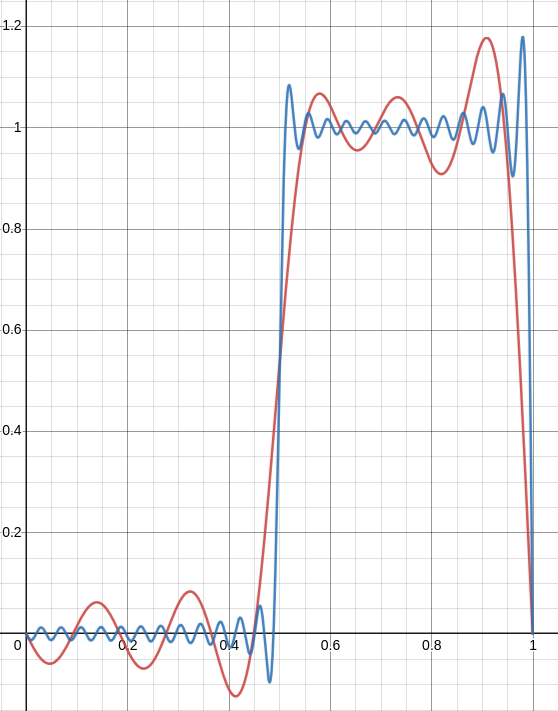
\includegraphics[width=0.5\textwidth]{u_0Approx.png}
\end{figure}

\begin{figure}[ht]
\caption{Approximations of $u_1$}
\centering
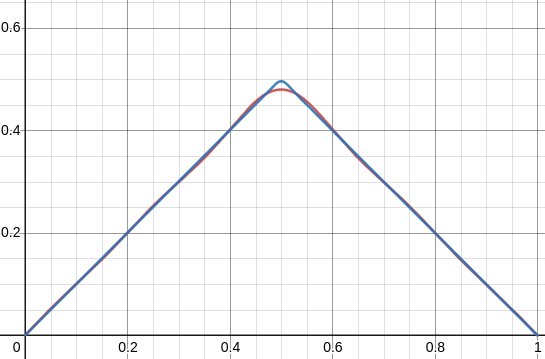
\includegraphics[width=0.5\textwidth]{u_1Approx.png}
\end{figure}

\begin{figure}[ht]
\caption{Approximations of $u_2$}
\centering
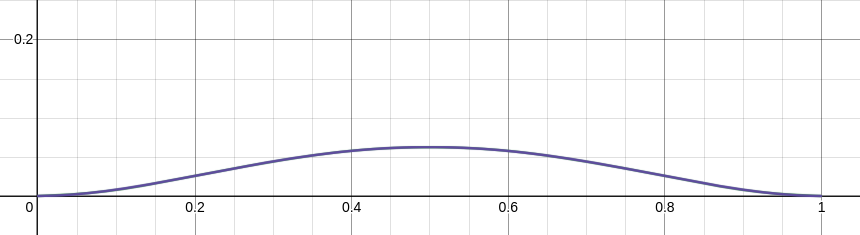
\includegraphics[width=0.5\textwidth]{u_2Approx.png}
\end{figure}

\section{Problem 3}
\textbf{Reminder:} Any closed subset of a compact set is compact.\\
\textbf{Solution for the exercise:}

We start with a bounded sequence of functions in $H^1$ i.e. $||u_k||_{H^1}\leq M$.
Without loss of generality we can assume $M=1$ i.e. $||u_k||_{H^1}\leq 1$.

Let $v_k=(v_k^1,v_k^2,\dots)\in l_2$ be the sequence of the Fourier coefficients of $u_k$.
Using problem 2 we know that $\sum_nn^2(v_k^n)^2\leq c$ and again WLOG we can
assume $c=1$ i.e. $\sum_nn^2(v_k^n)^2\leq 1$ which implies $|v_k^n|\leq
\frac{1}{n}$. And because the sequence $a_n=\frac{1}{n}$ is in $l_2$, then from
a result we saw in class and the previous reminder it follows that
$\overline{\{v_k\}}$ is compact in $L_2$. So there is a subsequence $v_{k_j}$
that is convergent to an element $v\in \overline{\{v_k\}}\subset l_2$. Using
the inverse Fourier transform on $v$ we get that there is a function $u\in L_2$
that satisfies: $\lim_{j\to\infty}||u_{k_j}-u||_{L_2}=0$, i.e.
$\overline{\{u_k\}}$ is compact.
\section{Problem 4}

\end{document}
